
\section{Introduction}
\label{sec:introduction}

Real-time collaborative editors allow authors to simultaneously write shared
documents~\cite{greenberg1994real}. Trending editors such as Google Docs rely on
central servers. They raise privacy issues since service providers take
advantage of their mediating position to observe all users and documents. They
also raise scalability issues for a server cannot handle the load of hundreds of
users. Yet, by their ease-of-usage, they became very popular.

% With centralization come privacy and scalability issues. To reconcile with the
% Internet working distributed without central authorities, editors start to get
% rid of such centrality point, which in turns solves privacy issues. Still
% scalability problem remains, and usability formerly provided by the Cloud is
% gone.

\CRATE is a distributed and decentralized \textsc{c}ollabo\textsc{rat}ive
\textsc{e}ditor providing scalable real-time editing capabilities directly
within web browsers. Users of heterogeneous devices are able to access to an
editing session as simply as clicking a URL (\emph{Uniform Resource Locator}).

Such simplicity is possible thanks to
WebRTC\footnote{\url{http://www.webrtc.org}}, a recent technology that enables
browser-to-browser communications. \CRATE builds an editing session using
\SPRAY~\cite{nedelec2015spray}, a random peer sampling
protocol~\cite{jelasity2007gossip} (RPS) built on top of WebRTC. Unlike prior
RPS, it provides each editor with a local neighbborhood table the size of which
automatically adapts to the editing session size. Since the propagation protocol
of messages~\cite{birman1999bimodal} extensively uses these tables, the network
traffic inherits from this scalability. Consequently, \CRATE adapts its
operation to the need of the editing session size.

To provide availability and responsiveness of documents, \CRATE uses the
optimistic replication scheme~\cite{saito2005optimistic}. Thus, each editor
replicates the document locally and directly performs operations on it. Changes
are spread to all editors using the aforementioned RPS. When the same set of
operations are applied by editors, the replicates converge to an equivalent
state allowing users to read the same document.  This property is called
\emph{strong eventual consistency}~\cite{bailis2013eventual}.  \CRATE uses a
data structure that avoids conflicting operations by
design~\cite{shapiro2011comprehensive}. It relieves users from the burden of
solving conflicts at the cost of additional metadata the size of which is kept
\TODO{reasonable} thanks to \LSEQ~\cite{nedelec2013lseq}. In particular, the
latter avoids any unaffordable distributed garbage-collection-like mechanism.

% To spread changes made on documents to the editing session, \CRATE firstly
% builds a network of browsers which is secondly used to disseminate messages in a
% scalable manner~\cite{birman1999bimodal}. Such feature is only allowed by the
% recent introduction of WebRTC\footnote{\url{http://www.webrtc.org}} as a
% browser-to-browser communication protocol. To build the network of browsers,
% \CRATE uses \SPRAY~\cite{nedelec2015spray}: a random peer sampling
% protocol~\cite{jelasity2007gossip} which provides each editor with a
% neighborhood table to communicate with. The size of the latter adapts to the
% editing session size automatically and without any global knowledge. The
% dissemination protocol built on top of it directly benefits from this
% property. Thus, traffic follows the needs of the editing session.

This demo paper
\begin{inparaenum}[(i)]
\item describes the aforementioned components that build \CRATE;
\item describes the setup of our live demo where people would get the
  opportunity to join an editing session and start the redaction of a document
  together. We hope to retrieve a meaningful document along with interesting
  measurements \TODO{confirming the results of our prior experiments performed
    on Grid'5000 involving up to 600 artifical editors typing.}
\end{inparaenum}

\TODO{The rest of this paper is organized as follow}:
Section~\ref{sec:architecture} details the overall architecture of \CRATE along
with its basic functioning. Section~\ref{sec:structure} describes the
distributed data structure that represents the
document. Section~\ref{sec:network} details the network building
operation. Section~\ref{sec:live} states the live experiment setup we
propose. Section~\ref{sec:conclusion} concludes.

\begin{figure*}
  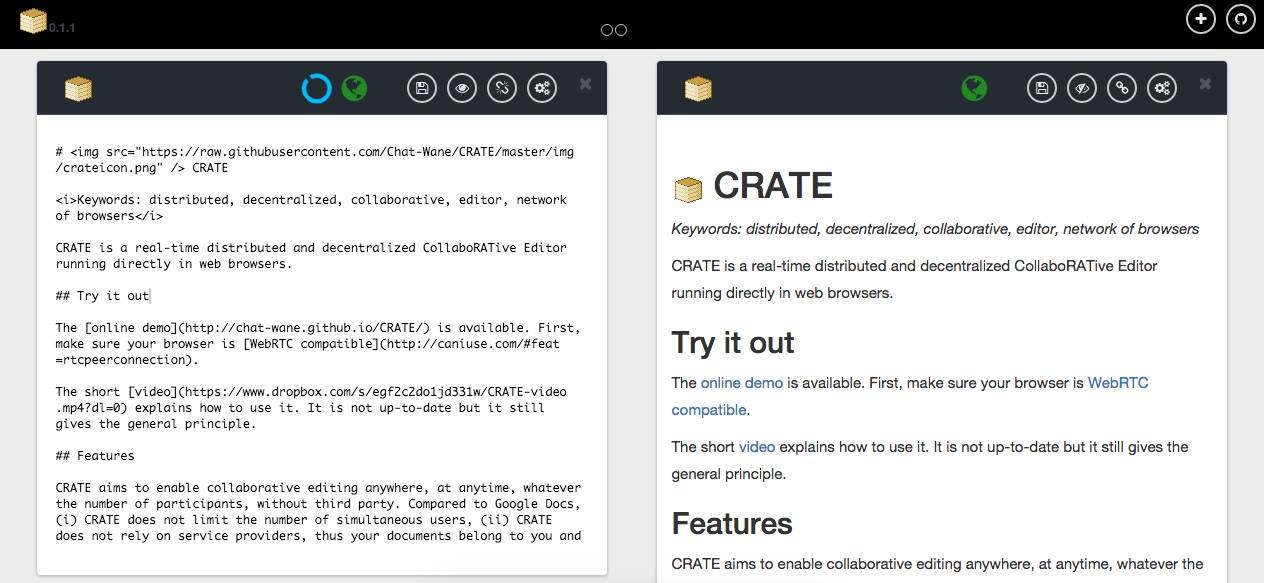
\includegraphics[width=\textwidth]{./img/screenshot.png}
  \caption{\label{img:screenshot} Screenshot of the web application containing
    two editors: on the left, a document is written in markdown language which
    is previewed on the right editor.}
\end{figure*}

%%% Local Variables:
%%% mode: latex
%%% TeX-master: "../paper"
%%% End:
